\documentclass[tikz,dvisvgm]{standalone}
\usetikzlibrary{shapes.geometric, arrows, positioning, fit}

\begin{document}
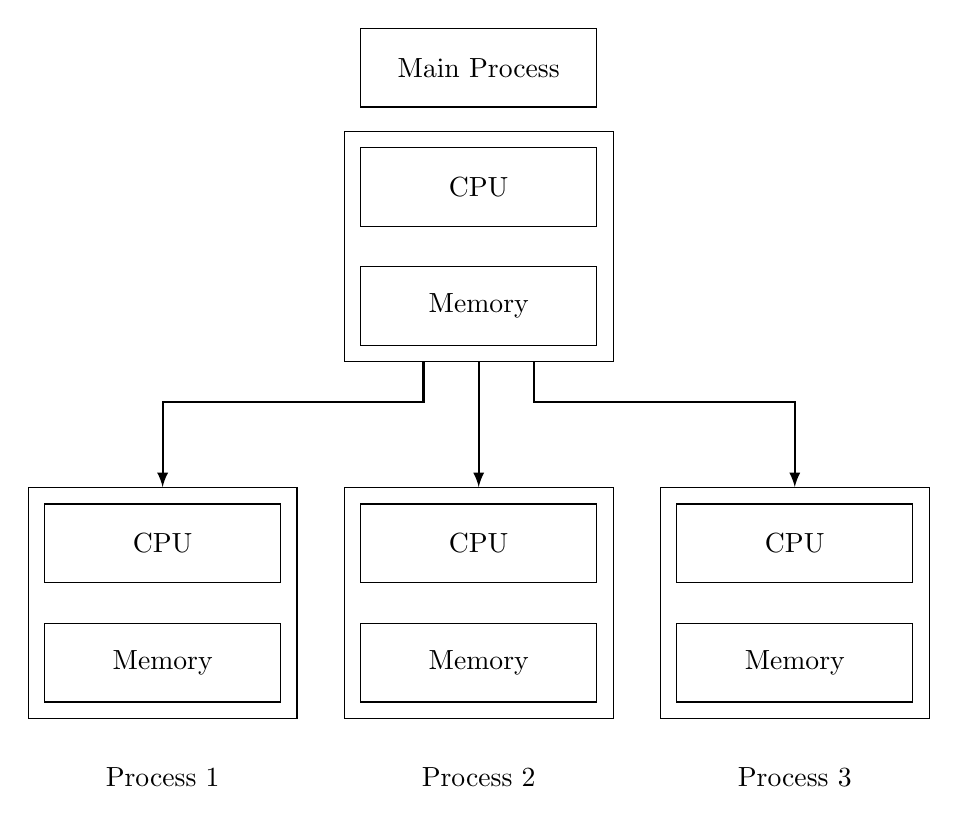
\begin{tikzpicture}[
    process/.style={rectangle, draw, minimum width=3cm, minimum height=1cm},
    thread/.style={rectangle, draw, minimum width=1cm, minimum height=0.5cm, fill=gray!20},
    arrow/.style={-latex, thick},
    dashedarrow/.style={->>>, double,thick, dashed},
    label/.style={font=\large\bfseries}
]

% Multiprocessing
\node[process] (main1) {Main Process};
\node[process, below=0.5cm of main1] (cpu1) {CPU};
\node[process, below=0.5cm of cpu1] (memory1) {Memory};

% Box around CPU and Memory in Multiprocessing
\node[draw, fit=(cpu1) (memory1), inner sep=0.2cm] (multiprocessing) {};

% Subprocesses
\node[process, below left=2cm and 1cm of memory1] (sub1cpu) {CPU};
\node[process, below=0.5cm of sub1cpu] (sub1mem) {Memory};
\node[draw, fit=(sub1cpu) (sub1mem), inner sep=0.2cm] (sub1box) {};
\node[below=0.5cm of sub1box] (sub1label) {Process 1};

\node[process, below=2cm of memory1] (sub2cpu) {CPU};
\node[process, below=0.5cm of sub2cpu] (sub2mem) {Memory};
\node[draw, fit=(sub2cpu) (sub2mem), inner sep=0.2cm] (sub2box) {};
\node[below=0.5cm of sub2box] (sub2label) {Process 2};

\node[process, below right=2cm and 1cm of memory1] (sub3cpu) {CPU};
\node[process, below=0.5cm of sub3cpu] (sub3mem) {Memory};
\node[draw, fit=(sub3cpu) (sub3mem), inner sep=0.2cm] (sub3box) {};
\node[below=0.5cm of sub3box] (sub3label) {Process 3};

% Connections
\coordinate [left=0.7cm of multiprocessing.south] (subwest);
\draw[arrow] (subwest) -- ++(0,-0.5) -| (sub1box.north);
\draw[arrow] (multiprocessing.south) --  (sub2box.north);
\coordinate [right=0.7cm of multiprocessing.south] (subeast);
\draw[arrow] (subeast) -- ++(0,-0.5) -| (sub3box.north);


\end{tikzpicture}
\end{document}